\documentclass[]{standalone}
%\usepackage{mathptmx}
%\renewcommand{\familydefault}{\rmdefault}
\usepackage[T1]{fontenc}
\usepackage[latin9]{inputenc}
\usepackage{siunitx}
\usepackage{array}
\usepackage{amsmath}
\usepackage{ifthen}
\usepackage{pgfplots}
\pgfplotsset{compat=1.14}
\usepackage{titling, graphicx}
\usepackage{tikz}
\usepackage{upgreek}
\usepackage{amsmath,amsthm}
\usepackage{strtikz}
\usetikzlibrary{shapes,arrows.meta,intersections,graphs,graphs.standard}
\usetikzlibrary{math,fit}
\usetikzlibrary{calc,intersections,through,backgrounds,decorations.pathmorphing}


\begin{document}
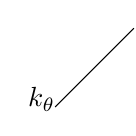
\begin{tikzpicture}
\rotspring[startx = 2cm,
starty = 3cm,
rotation = 90,
start rigid length = 0.5cm,
end rigid length = 0.5cm,
rotational spring diameter = 0.0004cm,
rotational spring cycle number = 3,
text = $k_{\theta}$]
\draw (0,0) -- (1cm,1cm);
\end{tikzpicture}
\end{document}